\chapter{Planteamiento del problema}
\addcontentsline{toc}{chapter}{Planteamiento del problema}

En la asignatura Desarrollo Basado en Agentes los alumnos, organizados en grupos de 4 o 5 alumnos, se conectan a un Laboratorio remoto de la UGR que está siempre disponible para los mismos. La arquitectura del servidor remoto puede apreciarse en la Figura \ref{fig:architecture}.

\begin{figure}[H]
    \centering
    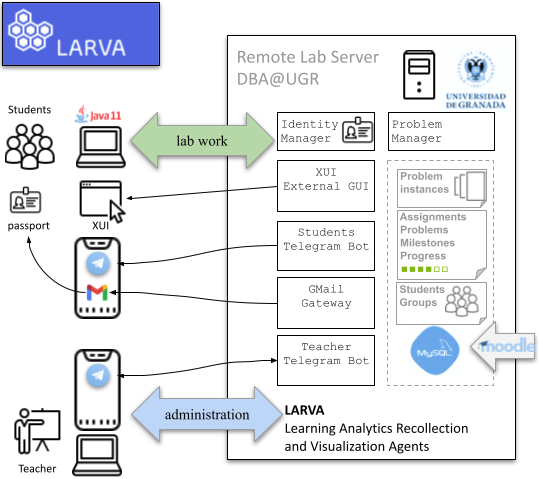
\includegraphics[width=0.60\textwidth]{LARVA2122Architecturec.png}
    \caption{Arquitectura del Servidor Remoto. Por un lado, contiene el laboratorio virtual para sistemas multiagente distribuidos. Además, los alumnos también pueden consultar su progreso y el de sus compañeros a través de un Bot de Telegram. Por otro lado, el profesor también puede conocer el número de objetivos conseguidos por cada uno de sus grupos de alumnos.}
    \label{fig:architecture}
\end{figure}

Este servidor contiene varios mundos virtuales y se encarga de registrar y almacenar las interacciones con él \cite{Vidal_2016}. Cada mundo virtual es una matriz cuadrada que representa espacios abiertos (en color blanco), obstáculos (en negro) y objetivos (en rojo) tal y como se muestra en la Figura \ref{fig:map}. Los agentes de los alumnos deben entrar en uno de esos mundos virtuales, percibir su vecindario, navegar a través de los espacios abiertos (empleando alguna clase de heurística exploratoria), evitar obstáculos y tratar de llegar al objetivo. En total, cada uno de los problemas planteados requieren de cinco pasos (o \emph{milestones}) hasta su consecución.

\begin{figure}[H]
    \centering
    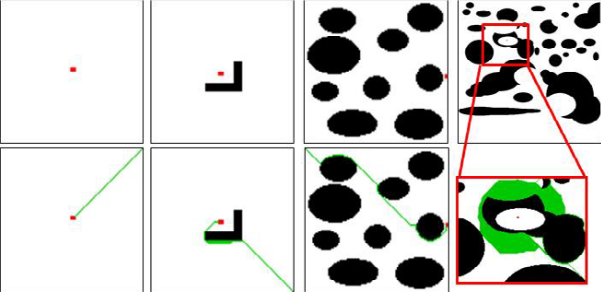
\includegraphics[width=0.60\textwidth]{virtualworlds.png}
    \caption{Alguno de los mapas que el alumnado debe resolver. Los agentes de los grupos de estudiantes deben acceder a uno de esos mundos y deben alcanzar los objetivos (coloreados en rojo) navengado a través del mundo y evitando los obstáculos (coloreados en negro). Alguno de los mundos no son resolubles porque el objetivo no se puede alcanzar con el objetivo de forzar a los agentes de los alumnos a razonar acerca de la irresolubilidad. Las posibles trayectorias están marcadas en verde.}
    \label{fig:map}
\end{figure}

La percepción del agente de su entorno es crítica para resolver estos mundos. En este laboratorio virtual los alumnos pueden configurar cuál de los siguientes sensores estarán enchufados en sus agentes (cualquier combinación de ellos):

\begin{itemize}
	\item Un \textbf{GPS} que indica al agente sus coordenadas $(x,y)$ en el mundo virtual.
	\item Un \textbf{sensor de batería}. Cada agente está alimentado con una batería cuya capacidad es limitada y cuya carga decrece conforme el agente realiza algún movimiento. La batería nunca debe ser vaciada por completo.
	\item Un \textbf{sensor radar} que informa al agente acerca de los tipos de celdas que lo rodean con una percepción local de 5x5 (observar Figura \ref{fig:sensorb}).
	\item Un \textbf{sensor escáner} que actúa como \emph{detector del objetivo} e indica al agente la distancia al objetivo medida desde cada una las celdas de su entorno 5x5 (observar Figura \ref{fig:sensorc}).
\end{itemize}

\begin{figure}[H]
\centering
\subfloat[]{\label{fig:sensora}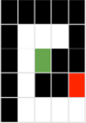
\includegraphics[width=0.10\textwidth]{sensora.png}}\qquad
\subfloat[]{\label{fig:sensorb}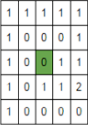
\includegraphics[width=0.10\textwidth]{sensorb.png}}\qquad
\subfloat[]{\label{fig:sensorc}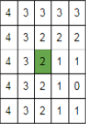
\includegraphics[width=0.10\textwidth]{sensorc.png}}%
\caption{Un agente (representado por una celda verde en el centro de cada figura) tiene una percepción local de su entorno: solamente percibe el entorno 5x5 de celdas colindantes. El Radar \ref{fig:sensorb} muestra dicho entorno 5x5 que rodea al agente e informa de si una celda está vacía (valor $0$), si hay un obstáculo (valor $1$) o de si hay un objetivo (valor $2$). El Escáner \ref{fig:sensorc} muestra la distancia de cada una de las celdas colindantes al objetivo.}
\label{fig:sensors}
\end{figure}

Basados en su percepción del mundo virtual, cada agente decidirá ejecutar alguna de las siguientes acciones en su entorno implementando cualquier heurística o proceso de búsqueda.

\begin{itemize}
	\item LOGIN. Entrar en cualquiera de los mundos virtuales.
	\item MOVE. Mover al agente a una de las $8$ celdas adyacentes y gastar una cierta cantidad de batería. Si la celda destino es un obstáculo o el agente se queda sin batería, el agente se rompe y se sale del mundo  virtual.
	\item REFUEL. El agente recarga completamente su batería. A los agentes se les permite recargar su batería tantas veces como deseen.
\end{itemize}